La mayor evidente diferencia entre el algoritmo presentado en la seccion \ref{sec:algoritmo-aternativo} y el algoritmo clásico es que en lugar de poder explorar transiciones entre estados completamente abstractos, la manera en la que explora las transiciones de la EPA implica que sólo está considerando ciertos caminos de métodos al evaluar cada transición.
Esto se debe a que en cada paso selecciona una par (método, estado abstracto) que no haya explorado ya, pero la exploración no se hace realmente desde todos los estados posibles que puedan abstraerse al estado abstracto, sino que se hace sobre un subconjunto de los estados que la herramienta pudo alcanzar hasta ese momento.

Consideremos el siguiente ejemplo, el contrato \texttt{BoundedStack}, cuyo código podemos ver en la figura \ref{fig:bounded-stack}:
Este contrato consiste en una implementación de simple implementación de una pila como estructura de datos, con la peculiaridad de que la pila cuenta con un tamaño máximo.
El método tiene sólo dós métodos externos: \textcolor{orange}{\texttt{push}} y \textcolor{orange}{\texttt{pop}}.
La EPA de este contrato por otro lado también es bastante sencilla, y la podemos ver en la imagen \ref{fig:bounded-stack-epa}.
Por fuera de los estados \textbf{init} y \textbf{vacio}, contamos con solo tres estados alcanzables, que son \textbf{\_push}, \textbf{\_pop} y \textbf{\_push\_pop}.
El estado \textbf{\_push} es corresponde con la pila vacía, y es el que se produce al deployear el contrato o luego de ejecutar \textcolor{orange}{\texttt{pop}} reiteradas veces.
Cuando la pila tiene elementos pero no está llena se corresponde con el estado \textbf{\_push\_pop}, al que se puede llegar tanto desde sí mismo, como desde \textbf{\_push} y desde \textbf{\_pop}.
Finalmente, el estado \textbf{\_pop} se corresponde con la pila llena, y se puede llegar tanto desde \textbf{\_push} (si el tamaño de la pila fuese uno) o desde \textbf{\_push\_pop}, pero no desde el constructor.
Notoriamente, a menos que el contrato sea deployeado con un tamaño máximo de cero, nunca será posible alcanzar el estado \textbf{\_vacio}.

Este es un buen ejemplo para observar la limitación introducida por el algoritmo alternativo al no explorar realmente todas las ejecuciones posibles de un método.
Como se representa en la figura \ref{fig:bounded-stack-bad-epa}, veremos que es posible que el análisis del \texttt{BoundedStack} por el algoritmo alternativo no pueda encontrar algunas de las transiciones presentes en la EPA, dependiendo del orden en el que elija ejecutar los métodos del contrato.
Para eso, tendremos que realizar manualmente la exploración que realizaría el algoritmo en este caso particular.
Observemos la figura \ref{fig:bounded-stack-bad-epa}.
Podemos llegar a ese resultado de la siguiente manera:
Consideremos que es lo que sucede cuando el algoritmo explora los estados alcanzables desde el constructor.
En efecto, como vimos en la EPA de \texttt{BoundedStack}, se pueden alcanzar los estados \textbf{\_push} y \textbf{vacio}.
Hasta ahora tenemos entonces $P_0 = \{\emptyset, \textbf{\_push}\}, S = \{\emptyset, \textbf{\_push}\}$ y que  $\Delta(s,m) = \emptyset$ para todos los $m$ y $s$.
Luego, el algoritmo elige un método de los disponibles a ejecutar al azar, que en este caso sería solamente \textcolor{orange}{\texttt{push}}.
Luego de ejecutar ese método veremos que son alcanzables desde \textbf{\_push} los estados \textbf{\_push\_pop} (con la restricción de que el tamaño de la pila sea mayor a uno) y \textbf{\_pop} (con la restricción de que el tamaño de la pila sea exactamente uno).
En este punto, $P_0 = \{\emptyset, \textbf{\_push}\}, S = \{\emptyset, \textbf{\_push}, \textbf{\_push\_pop}, \textbf{\_pop}\}$ y  $\Delta(\textbf{\_push},\textcolor{orange}{\texttt{push}}) = \{\textbf{\_push\_pop}, \textbf{\_pop}\}$.

Ahora, este es el punto en el que el próximo paso de la exploración del algoritmo cambiará en el resultado final de la abstracción construida.
Por un lado, podemos elegir explorar \textcolor{orange}{\texttt{pop}} desde \textbf{\_push\_pop} y \textbf{\_pop}, marcando ambos pares como ya explorados, o explorar \textcolor{orange}{\texttt{push}} desde \textbf{\_push\_pop} y dejar la exploración de \textcolor{orange}{\texttt{push}} para más adelante.
Si continuamos la ejecución suponiendo que en este paso se elige explorar \textcolor{orange}{\texttt{pop}}, descubriremos dos transiciones nuevas: de \textbf{\_push\_pop} a \textbf{\_push} mediante \textcolor{orange}{\texttt{pop}} y de \textbf{\_pop} a \textbf{\_push} mediante \textcolor{orange}{\texttt{pop}} también.
Nos puede llamar la atención que desde los estados (concretos) que elegimos para explorar la ejecución de \textcolor{orange}{\texttt{pop}} hay dos transiciones que no podemos ver: de de \textbf{\_pop} a \textbf{\_push\_pop} mediante \textcolor{orange}{\texttt{pop}} y de de \textbf{\_push\_pop} a \textbf{\_push\_pop} mediante \textcolor{orange}{\texttt{pop}}.
Estas se deben a que en este momento todos los estados concretos que estamos considerando tienen su tamaño real de la pila en 1.
Sin embargo, el algoritmo no presta atención a cuál fue la traza de métodos ejecutada para llegar hasta acá, por lo que marca a ambas tuplas $(\textbf{\_push\_pop},\textcolor{orange}{\texttt{pop}})$ y $(\textbf{\_pop},\textcolor{orange}{\texttt{pop}})$ como ya exploradas.
Esto significa que la función de transición $\Delta$ quedará definida en $\Delta(\textbf{\_push\_pop},\textcolor{orange}{\texttt{pop}}) = \textbf{\_push}$ y $\Delta(\textbf{\_pop},\textcolor{orange}{\texttt{pop}}) = \textbf{\_push}$ y luego procedirá con la ejecución hasta finalizar el algoritmo con (al menos) esas dos transiciones faltantes.

\begin{lstlisting}[language=Solidity, label={fig:bounded-stack}, caption={Contrato Inteligente \texttt{BoundedStack} en Solidity},captionpos=b]
pragma solidity ^0.5.17;
contract SizedStack {
    uint256 public size;
    uint256 public maxSize;
    uint256[] internal_arr;
    constructor() public {
        maxSize = 10;
        size = 0;
    }
    function isEmpty() public view returns (bool) {
        return size == 0;
    }
    function top() public view returns (uint256) {
        require(!isEmpty());
        return internal_arr[size - 1];
    }
    function push(uint256 new_elem) public {
        require(size < maxSize);
        internal_arr.push(new_elem);
        size += 1;
    }
    function pop() public returns (uint256) {
        require(!isEmpty());
        uint256 was = top();
        internal_arr.pop();
        size -= 1;
        return was;
    }
}
\end{lstlisting}

\begin{figure}
    \centering
    \begin{subfigure}{0.45\textwidth}
        {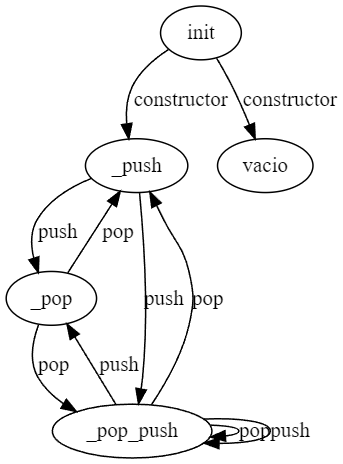
\includegraphics[width=\textwidth]{figs/bounded-stack-good-epa.png}}
        \caption{Enabledness Preserving Abstraction del contrato \texttt{BoundedStack}}
        \label{fig:bounded-stack-epa}
    \end{subfigure}
    \hfill
    \begin{subfigure}{0.45\textwidth}
        {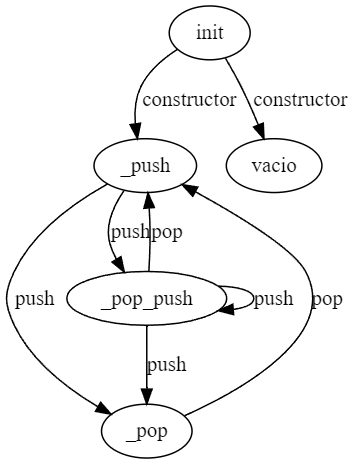
\includegraphics[width=\textwidth]{figs/bonded-stack-bad-epa.png}}
        \caption{EPA errónea del contrato \texttt{BoundedStack} generada por el algoritmo alternativo}
        \label{fig:bounded-stack-bad-epa}
    \end{subfigure}
\end{figure}


%A pesar de que Manticore permita el uso de valores simbólicos para el parámetro \texttt{(msg.sender)} las limitaciones de la herramienta exigen que se defina cada account individualmente para que sea considerada en el estado de la blockchain.
Las limitaciones de la herramienta exigen que el parámetro \texttt{(msg.sender)}, a pesar de que pueda ser simbólico, se corresponda con una \textit{account} definida explícitamente por el usuario.
Por esto en la simulación contamos con un número fijo de \textit{accounts}, asignando variables simbólicas únicamente la información asociada a ellas (Dirección, Balance, etc).

Al evaluar el funcionamiento del prototipo buscamos responder las siguientes preguntas:
\begin{enumerate}
    \item ¿Son correctas las EPAs que genera el prototipo?
    \item ¿Cuál es su performance en contratos inteligentes reales?
\end{enumerate}
Para responder estas preguntas, pusimos el prototipo a prueba contra algunos contratos provenientes de Microsoft Azure Blockchain Workbench \cite{azure-benchmark}.
Este conjunto de contratos había sido utilizado anteriormente por Godoy et al. \cite{predicate-abstraction-for-smart-contract-validation}, por lo que convenientemente ya contamos con las EPAs correspondientes.
Ejecutamos el prototipo cinco veces, obteniendo el promedio de su tiempo de ejecución sobre los contratos seleccionados y luego corroboramos que la EPA generada fuera isomórfica a la obtenida en los estudios anteriores.
%Además, pusimos a prueba la cantidad de accounts necesarias para el funcionamiento del prototipo.
Los resultados intermedios indicaron que para los contratos propuestos era suficiente realizar la simulación con dos \textit{accounts}, por lo que utilizamos esa cantidad para los experimentos.
Los resultados de esta experimentación se ven resumidos en la tabla \ref{tab:resultados}.
El prototipo generó EPAs correctas en todos los casos.
Sin embargo, el tiempo de cálculo es de entre media y casi tres horas, considerando incluso que los ejemplos utilizados son relativmente pequeños.
Algunos resultados intermedios indican que este tiempo es consumido principalmente por Manticore para la generación de \textit{path conditions}.
Debido a la rigurosidad con la que emula Manticore el comportamiento de la blockchain, la herramienta demora incluso para la ejecución simbólica de transiciones sencillas.

\vspace{-2.2em}

\begin{table}
    %\begin{adjustwidth}{-0.5in}{-0.5in}% adjust the L and R margins by 1 inch
    \caption{Resumen de la experimentación. \textbf{LOC} es cantidad de lineas de código, \textbf{Tiempo de ejecución} es el promedio del tiempo de ejecución medido en minutos, $\boldsymbol{\sigma}$ es el desvío estandard medido en segundos y \textbf{¿Es correcto?} indica si la EPA generada es isomorfa con la provista anteriormente.}\label{tab:resultados}
    \begin{tabular}{|l|l|l|l|l|}
        \hline
        Contrato                  & LOC & Tiempo de ejecución (min) & $\sigma$ (s) & ¿Es correcto? \\
        \hline
        DefectiveComponentCounter & 33  & $29$                      & $7$          & Sí            \\
        SimpleMarketplace         & 66  & $186$                     & $800$        & Sí            \\
        BasicProvenance           & 48  & $40$                      & $6$          & Sí            \\
        RoomThermostat            & 48  & $138$                     & $600$        & Sí            \\
        \hline
    \end{tabular}
    %\end{adjustwidth}
\end{table}
